\section{Preventivo}
Per descrivere come il gruppo \emph{TechSWEave} utilizzerà le risorse a sua disposizione, abbiamo stilatto delle tabelle orarie con la suddivisione dei ruoli, uttilizzando le seguenti sigle:
\begin{itemize}
    \item \textbf{Re: }\emph{Responsabile};
    \item \textbf{Am: }\emph{Amministratore}
    \item \textbf{An: }\emph{Analista};
    \item \textbf{Pt: }\emph{Progettista};
    \item \textbf{Pr: }\emph{Programmatore};
    \item \textbf{Ve: }\emph{Verificatore};
\end{itemize}

\subsection{Fase di Analisi}
    \subsubsection{Prospetto orario}
    In questa fase la distribuzione oraria è la seguente:
    %fare tabella e istogramma 
    %---------------------

    \begin{center}
        \begin{table}[ht!]
            \centering
            \rowcolors{2}{logo!10}{logo!40}
            \renewcommand{\arraystretch}{1.8}
            \begin{tabular}{p{100px} p{20px} p{20px} p{20px} p{20px} p{20px} p{20px} p{50px} }
                \rowcolor{logo!70} \textbf{Nominativo} & \textbf{Re} & \textbf{Am} & \textbf{An} & \textbf{Pt} & \textbf{Pr} & \textbf{Ve} & \textbf{Ore totali}\\
                Marco Barbaresco & - & 10 & 10 & - & - & 15 & 35\\
                Samuele De Simone & 8 & - & 17 & - & - & 10 & 35\\
                Nicolò Giaccone & - & 7 & 21 & - & - & 7 & 35\\
                Amedeo Meggiolaro & - & - & 18 & - & - & 17 & 35\\
                Tito Scurati & - & 8 & 12 & - & - & 15 & 35\\
                Simone Urbani & 6 & 10 & 8 & - & - & 11 & 35\\
                Manuel Varo & 7 & - & 12 & - & - & 16 & 35\\
                Ore totati di ruolo & 21 & 35 & 98 & - & - & 91 & 245\\
            \end{tabular}
        \end{table}
    \end{center}

    \pagebreak

    \begin{figure}[!h]
            \caption{Istogramma orari suddivisione dei ruoli}
            \vspace{5px}
            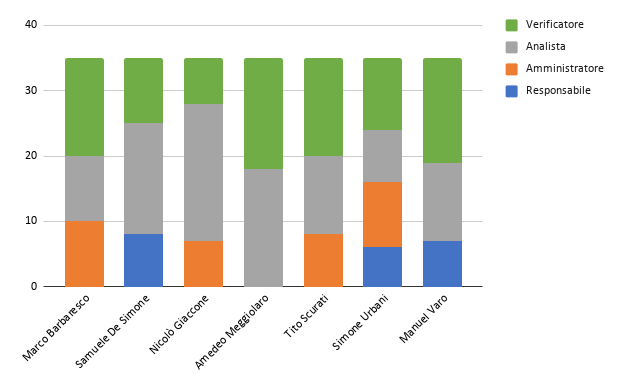
\includegraphics[scale=0.6]{../../../Images/Diagrammi/Istogrammi/ore analisi.png}
            \centering
        \end{figure}
    \subsubsection{Prospetto economico}
    In questa fase i costi da affrontare per ogni ruolo sono i seguenti:
    %fare tabella e istogramma 
    %---------------------
    \begin{center}
        \begin{table}[ht!]
            \centering
            \rowcolors{2}{logo!10}{logo!40}
            \renewcommand{\arraystretch}{1.8}
            \begin{tabular}{p{75px} p{20px} p{30px} }
                \rowcolor{logo!70} \textbf{Ruolo} & \textbf{Ore} & \textbf{Costo}\\
                Responsabile & 21 & 630 \\
                Amministratore & 35 & 700 \\
                Analista & 98 & 2450 \\
                Progettista & - & - \\
                Programmatore & - & - \\
                Verificatore & 91 & 1365  \\
                Totale & 245 & 5145  \\
            \end{tabular}
        \end{table}
    \end{center}
    \pagebreak
    \begin{figure}[!h]
        \caption{aerogramma ore per ruolo}
        \vspace{5px}
        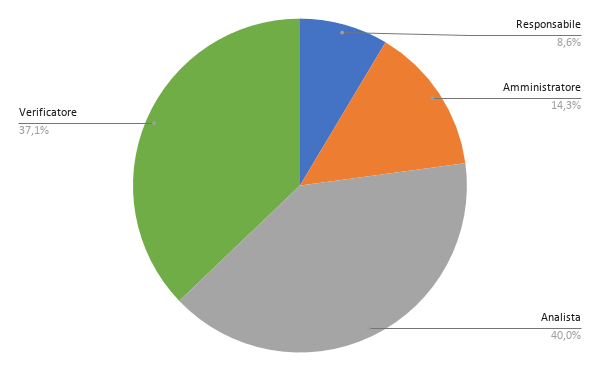
\includegraphics[scale=0.5]{../../../Images/Diagrammi/Diagramma a torta/ore analisi.png}
        \centering
    \end{figure}

    
\subsection{Fase di Consolidamento dei requisiti}
    \subsubsection{Prospetto orario}
    In questa fase la distribuzione oraria è la seguente:
    %fare tabella e istogramma 
    %---------------------

        \begin{center}
            \begin{table}[ht!]
                \centering
                \rowcolors{2}{logo!10}{logo!40}
                \renewcommand{\arraystretch}{1.8}
                \begin{tabular}{p{100px} p{20px} p{20px} p{20px} p{20px} p{20px} p{20px} p{50px} }
                    \rowcolor{logo!70} \textbf{Nominativo} & \textbf{Re} & \textbf{Am} & \textbf{An} & \textbf{Pt} & \textbf{Pr} & \textbf{Ve} & \textbf{Ore totali}\\
                    Marco Barbaresco & - & - & 2 & - & - & 4 & 6\\
                    Samuele De Simone & 4 & - & - & - & - & 2 & 6\\
                    Nicolò Giaccone & - & - & 6 & - & - & - & 6\\
                    Amedeo Meggiolaro & - & - & - & - & - & 6 & 6\\
                    Tito Scurati & - & - & 6 & - & - & - & 6\\
                    Simone Urbani & - & 6 & - & - & - & - & 6\\
                    Manuel Varo & - & - & 2 & - & - & 4 & 6\\
                    Ore totati di ruolo & 4 & 6 & 16 & - & - & 16 & 42\\
                \end{tabular}
            \end{table}
        \end{center}
        \pagebreak

        \begin{figure}[!h]
            \caption{Istogramma orari suddivisione dei ruoli}
            \vspace{5px}
            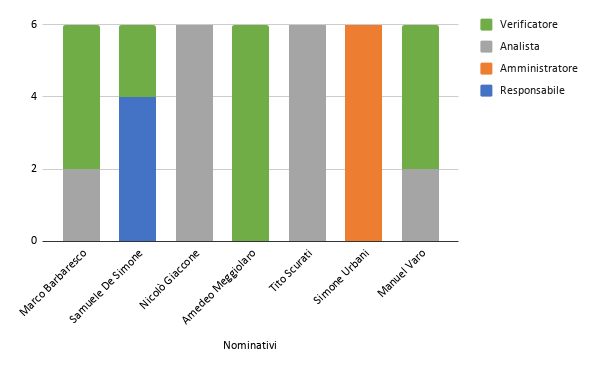
\includegraphics[scale=0.6]{../../../Images/Diagrammi/Istogrammi/ore requisiti.png}
            \centering
        \end{figure}

    \subsubsection{Prospetto economico}
In questa fase i costi da affrontare per ogni ruolo sono i seguenti:
%fare tabella e istogramma 
%---------------------
        \begin{center}
            \begin{table}[ht!]
                \centering
                \rowcolors{2}{logo!10}{logo!40}
                \renewcommand{\arraystretch}{1.8}
                \begin{tabular}{p{75px} p{20px} p{30px}}
                    \rowcolor{logo!70} \textbf{Ruolo} & \textbf{Ore} & \textbf{Costo}\\
                    Responsabile & 4 & 120 \\
                    Amministratore & 6 & 120 \\
                    Analista & 16 & 400 \\
                    Progettista & - & - \\
                    Programmatore & - & - \\
                    Verificatore & 16 & 240  \\
                    Totale & 42 & 880 \\
                \end{tabular}
            \end{table}
        \end{center}
        \pagebreak

        \begin{figure}[!h]
            \caption{aerogramma ore requisiti per ruolo}
            \vspace{5px}
            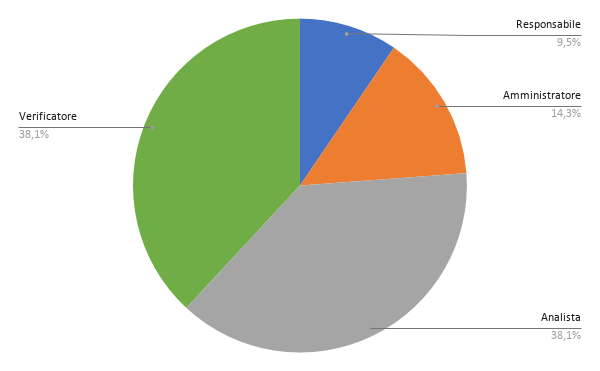
\includegraphics[scale=0.5]{../../../Images/Diagrammi/Diagramma a torta/ore requisiti.png}
            \centering
        \end{figure}



\subsection{Fase di Progettazione architetturale}
    \subsubsection{Prospetto orario}
    In questa fase la distribuzione oraria è la seguente:
    %fare tabella e istogramma 
    %---------------------
        \begin{center}
            \begin{table}[ht!]
                \centering
                \rowcolors{2}{logo!10}{logo!40}
                \renewcommand{\arraystretch}{1.8}
                \begin{tabular}{p{100px} p{20px} p{20px} p{20px} p{20px} p{20px} p{20px} p{50px} }
                    \rowcolor{logo!70} \textbf{Nominativo} & \textbf{Re} & \textbf{Am} & \textbf{An} & \textbf{Pt} & \textbf{Pr} & \textbf{Ve} & \textbf{Ore totali}\\
                    Marco Barbaresco & - & - & 6 & 13 & 5 & 4 & 28\\
                    Samuele De Simone & - & - & 10 & - & 6 & 12 & 28\\
                    Nicolò Giaccone & - & 7 & - & 15 & 6 & - & 28\\
                    Amedeo Meggiolaro & 5 & - & - & 12 & 3 & 8 & 28\\
                    Tito Scurati & 10 & 7 & - & 11 & - & - & 28\\
                    Simone Urbani & - & - & 6 & 12 & - & 10 & 28\\
                    Manuel Varo & - & 5 & 8 & - & 6 & 9 & 28\\
                    Ore totati di ruolo & 15 & 19 & 30 & 63 & 26 & 43 & 196\\
                \end{tabular}
            \end{table}
        \end{center}
        \pagebreak
        
        \begin{figure}[!h]
            \caption{Istogramma orari suddivisione dei ruoli}
            \vspace{5px}
            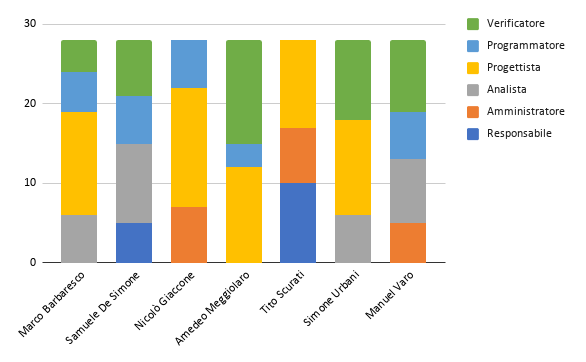
\includegraphics[scale=0.6]{../../../Images/Diagrammi/Istogrammi/ore architettura.png}
            \centering
        \end{figure}
    \subsubsection{Prospetto economico}
    In questa fase i costi da affrontare per ogni ruolo sono i seguenti:
    %fare tabella e istogramma 
    %---------------------
        \begin{center}
            \begin{table}[ht!]
                \centering
                \rowcolors{2}{logo!10}{logo!40}
                \renewcommand{\arraystretch}{1.8}
                \begin{tabular}{p{75px} p{20px} p{30px}}
                    \rowcolor{logo!70} \textbf{Ruolo} & \textbf{Ore} & \textbf{Costo}\\
                    Responsabile & 15 & 450 \\
                    Amministratore & 19 & 380 \\
                    Analista & 30 & 750 \\
                    Progettista & 63 & 1368 \\
                    Programmatore & 26 & 390 \\
                    Verificatore & 43 & 645  \\
                    Totale & 196 & 4001 \\
                \end{tabular}
            \end{table}
        \end{center}
        \pagebreak

        \begin{figure}[!h]
            \caption{aerogramma ore requisiti per ruolo}
            \vspace{5px}
            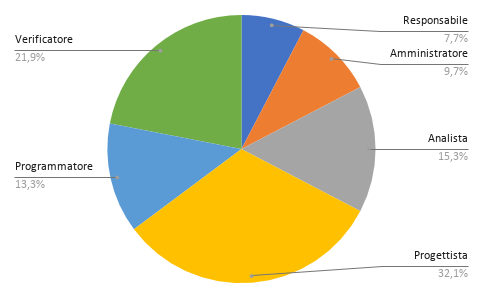
\includegraphics[scale=0.5]{../../../Images/Diagrammi/Diagramma a torta/ore architettura.png}
            \centering
        \end{figure}


\subsection{Fase di dettaglio e codifica}
    \subsubsection{Prospetto orario}
    In questa fase la distribuzione oraria è la seguente:
    %fare tabella e istogramma 
    %---------------------
        \begin{center}
            \begin{table}[ht!]
                \centering
                \rowcolors{2}{logo!10}{logo!40}
                \renewcommand{\arraystretch}{1.8}
                \begin{tabular}{p{100px} p{20px} p{20px} p{20px} p{20px} p{20px} p{20px} p{50px} }
                    \rowcolor{logo!70} \textbf{Nominativo} & \textbf{Re} & \textbf{Am} & \textbf{An} & \textbf{Pt} & \textbf{Pr} & \textbf{Ve} & \textbf{Ore totali}\\
                    Marco Barbaresco & 9 & - & - & 14 & 12 & 15 & 50\\
                    Samuele De Simone & - & 8 & - & 18 & 13 & 11 & 50\\
                    Nicolò Giaccone & 8 & - & - & 8 & 20 & 14 & 50\\
                    Amedeo Meggiolaro & 6 & 5 & - & 9 & 12 & 18 & 50\\
                    Tito Scurati & - & 9 & - & 14 & 18 & 9 & 50\\
                    Simone Urbani & 8 & - & - & 14 & 16 & 12 & 50\\
                    Manuel Varo & - & 12 & - & 13 & 9 & 16 & 50\\
                    Ore totati di ruolo & 31 & 34 & 0 & 90 & 100 & 95 & 350\\
                \end{tabular}
            \end{table}
        \end{center}
        \pagebreak
        
        \begin{figure}[!h]
            \caption{Istogramma orari suddivisione dei ruoli}
            \vspace{5px}
            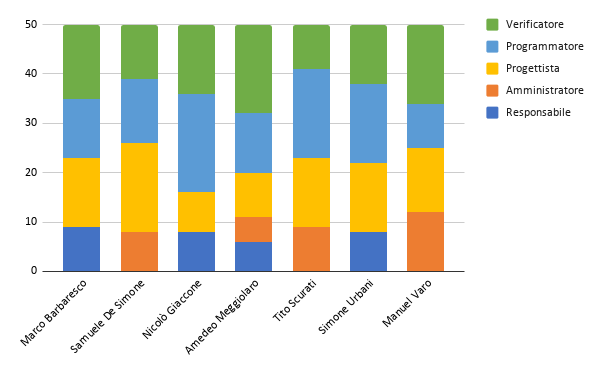
\includegraphics[scale=0.6]{../../../Images/Diagrammi/Istogrammi/ore codifica.png}
            \centering
        \end{figure}
    \subsubsection{Prospetto economico}
    In questa fase i costi da affrontare per ogni ruolo sono i seguenti:
    %fare tabella e istogramma 
    %---------------------
        \begin{center}
            \begin{table}[ht!]
                \centering
                \rowcolors{2}{logo!10}{logo!40}
                \renewcommand{\arraystretch}{1.8}
                \begin{tabular}{p{75px} p{20px} p{30px}}
                    \rowcolor{logo!70} \textbf{Ruolo} & \textbf{Ore} & \textbf{Costo}\\
                    Responsabile & 31 & 930 \\
                    Amministratore & 34 & 680 \\
                    Analista & - & - \\
                    Progettista & 90 & 1980 \\
                    Programmatore & 100 & 1500 \\
                    Verificatore & 95 & 1425  \\
                    Totale & 350 & 6515 \\
                \end{tabular}
            \end{table}
        \end{center}
        \pagebreak
            
        \begin{figure}[!h]
            \caption{aerogramma ore requisiti per ruolo}
            \vspace{5px}
            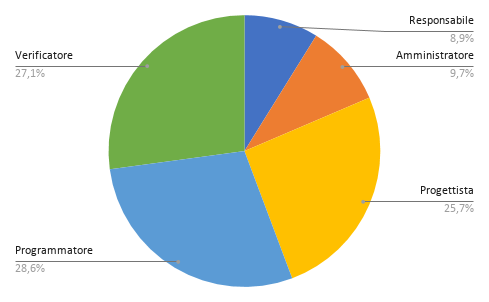
\includegraphics[scale=0.5]{../../../Images/Diagrammi/Diagramma a torta/ore codifica.png}
            \centering
        \end{figure}  



\subsection{Fase di Validazione e collaudo}
    \subsubsection{Prospetto orario}
    In questa fase la distribuzione oraria è la seguente:
    %fare tabella e istogramma 
    %---------------------
        \begin{center}
            \begin{table}[ht!]
                \centering
                \rowcolors{2}{logo!10}{logo!40}
                \renewcommand{\arraystretch}{1.8}
                \begin{tabular}{p{100px} p{20px} p{20px} p{20px} p{20px} p{20px} p{20px} p{50px} }
                    \rowcolor{logo!70} \textbf{Nominativo} & \textbf{Re} & \textbf{Am} & \textbf{An} & \textbf{Pt} & \textbf{Pr} & \textbf{Ve} & \textbf{Ore totali}\\
                    Marco Barbaresco & - & 8 & - & 2 & - & 10 & 20\\
                    Samuele De Simone & 4 & - & - & - & 7 & 9 & 20\\
                    Nicolò Giaccone & - & 5 & - & 6 & - & 9 & 20\\
                    Amedeo Meggiolaro & - & - & - & 12 & 8 & - & 20\\
                    Tito Scurati & 6 & - & - & - & 12 & 2 & 20\\
                    Simone Urbani & - & 6 & - & - & 10 & 4 & 20\\
                    Manuel Varo & 10 & - & - & - & 4 & 6 & 20\\
                    Ore totati di ruolo & 20 & 19 & 0 & 20 & 41 & 40 & 140\\
                \end{tabular}
            \end{table}
        \end{center}
        \pagebreak

        \begin{figure}[!h]
            \caption{Istogramma orari suddivisione dei ruoli}
            \vspace{5px}
            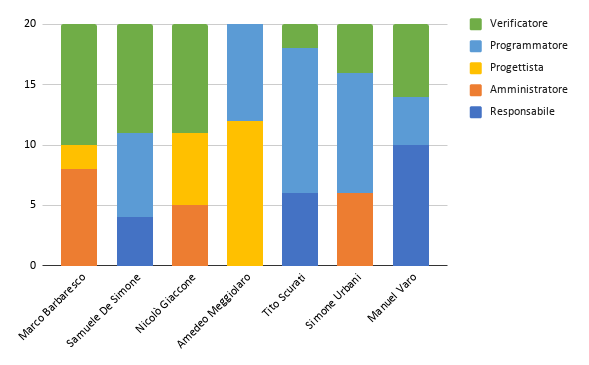
\includegraphics[scale=0.6]{../../../Images/Diagrammi/Istogrammi/ore validificazione.png}
            \centering
        \end{figure}
    \subsubsection{Prospetto economico}
    In questa fase i costi da affrontare per ogni ruolo sono i seguenti:
    %fare tabella e istogramma 
    %---------------------

        \begin{center}
            \begin{table}[ht!]
                \centering
                \rowcolors{2}{logo!10}{logo!40}
                \renewcommand{\arraystretch}{1.8}
                \begin{tabular}{p{75px} p{20px} p{30px}}
                    \rowcolor{logo!70} \textbf{Ruolo} & \textbf{Ore} & \textbf{Costo}\\
                    Responsabile & 20 & 600 \\
                    Amministratore & 19 & 380 \\
                    Analista & - & - \\
                    Progettista & 20 & 440 \\
                    Programmatore & 41 & 615 \\
                    Verificatore & 40 & 600  \\
                    Totale & 140 & 2635 \\
                \end{tabular}
            \end{table}
        \end{center}
        \pagebreak

        \begin{figure}[!h]
            \caption{aerogramma ore requisiti per ruolo}
            \vspace{5px}
            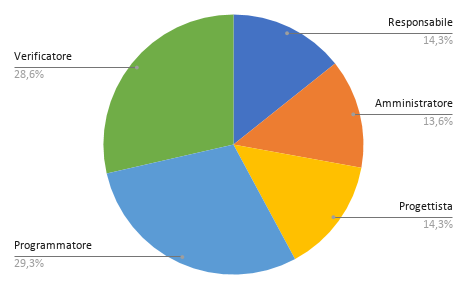
\includegraphics[scale=0.5]{../../../Images/Diagrammi/Diagramma a torta/ore validificazione.png}
            \centering
        \end{figure}  


\subsection{Riepologo}
    \subsubsection{Ore totali}
        \subsubsubsection{Suddivisione lavoro}
        Nella tabella sono riportate il totale delle ore del progetto, sono presenti sia le ore di investimento che quelle rendicontate a carico del commitente:
        %fare tabella e istogramma 
        %---------------------    
        \begin{figure}[!h]
            \caption{Istogramma orari suddivisione dei ruoli}
            \vspace{5px}
            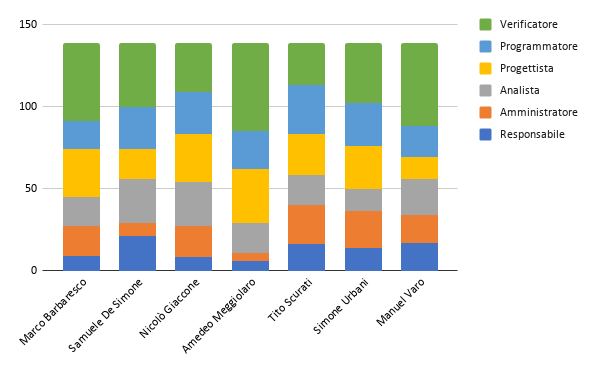
\includegraphics[scale=0.6]{../../../Images/Diagrammi/Istogrammi/ore totali.png}
            \centering
        \end{figure}

        \subsubsubsection{Prospetto economico}
        I costi da affrontare per ogni ruolo sono i seguenti:
        %fare tabella e istogramma 
        %---------------------   
        \begin{figure}[!h]
            \caption{Istogramma orari suddivisione dei ruoli}
            \vspace{5px}
            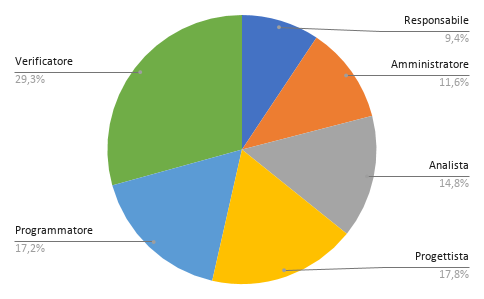
\includegraphics[scale=0.5]{../../../Images/Diagrammi/Diagramma a torta/ore totali.png}
            \centering
        \end{figure}
    \subsubsection{Ore rendicontate}
        \subsubsubsection{Suddivisione lavoro}
        Le ore rendicontante sono riportate nella seguente tabella:

        \begin{figure}[!h]
            \caption{Istogramma orari suddivisione dei ruoli}
            \vspace{5px}
            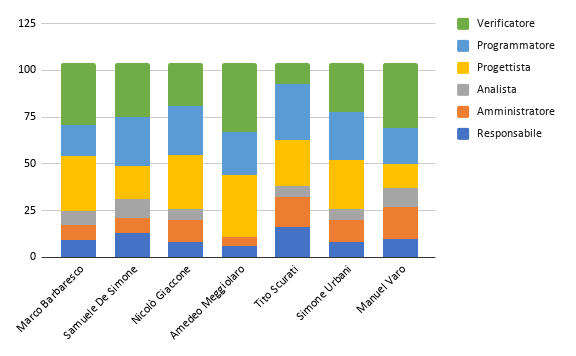
\includegraphics[scale=0.6]{../../../Images/Diagrammi/Istogrammi/ore rendicontate.png}
            \centering
        \end{figure}
        \subsubsubsection{Prospetto economico}
        Il totale rendicontato dei costi da affrontare per ogni ruolo è:
        %mettere tabella 

        \begin{figure}[!h]
            \caption{Istogramma orari suddivisione dei ruoli}
            \vspace{5px}
            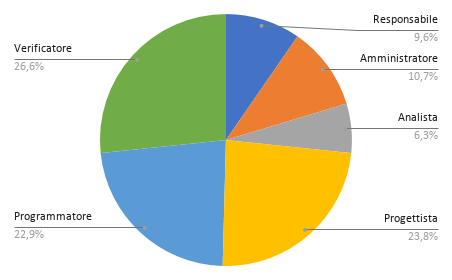
\includegraphics[scale=0.5]{../../../Images/Diagrammi/Diagramma a torta/ore rendicontate.png}
            \centering
        \end{figure}